\documentclass[12pt, conference]{IEEEtran}
\hyphenation{op-tical net-works semi-conduc-tor}
\usepackage{graphicx}
\graphicspath{{figures/}}
\usepackage{fancyhdr}
\usepackage{url}
\usepackage{textcomp}
\usepackage{amsmath}
\usepackage{listings}
\usepackage{algorithm}
\usepackage{algorithmic}
\usepackage{lipsum}
\usepackage{caption}
\usepackage{subcaption}
\usepackage{pdfpages}
\usepackage{bookmark}
\usepackage[normalem]{ulem}
\def\code#1{\texttt{#1}}
\usepackage{pdflscape}
\useunder{\uline}{\ul}{}
\usepackage{titlesec}


\titleformat{\section}
  {\normalfont\center\fontsize{13}{15}\bfseries\scshape}{\thesection}{0.5em}{}

\pagestyle{fancy}
\fancyhf{}
\lhead{\textsc{IBM: Data Science\\Professional Certificate}}
\rhead{\textsc{Applied Data Science Capstone:\\The Battle of the Neighbourhoods}}
\rfoot{Page \thepage\ }


\begin{document}
\onecolumn

%----------------------------------------------------------------------------------------

%----------------------------------------------------------------------------------------
%	IF NO TITLE PAGE
%----------------------------------------------------------------------------------------
%
% paper title
% Titles are generally capitalized except for words such as a, an, and, as,
% at, but, by, for, in, nor, of, on, or, the, to and up, which are usually
% not capitalized unless they are the first or last word of the title.
% Linebreaks \\ can be used within to get better formatting as desired.
% Do not put math or special symbols in the title.
%
\title{Applied Data Science Capstone:\\
The Battle of the Neighbourhoods}



% author names and affiliations
% use a multiple column layout for up to three different
% affiliations
\author{\IEEEauthorblockN{Kishan Narotam 
\IEEEauthorblockA{\url{https://knarotam.github.io/}\\
15/01/2021}}}
%\and
%\IEEEauthorblockN{Homer Simpsons}
%\IEEEauthorblockA{Twentieth Century Fox\\
%Springfield, USA\\
%Email: homer@thesimpsons.com}
%}
% make the title area
\maketitle

%----------------------------------------------------------------------------------------

%----------------------------------------------------------------------------------------
%	MAIN BODY OF REPORT
%----------------------------------------------------------------------------------------

\section{\textbf{Introduction}}
\label{sec: Introduction}
A venture capitalist is known as a private equity investor who seeks opportunity in high-growth potential companies such as small businesses and startups in exchange for a stake in the respective company. The risk-reward factor of investing in these companies can be drastic, and if invested correctly can yield a substantial return for the investor. Venture capital firms began in the United States in the early to mid-1900s and has continued to grow exponentially as the world evolved through the Dot-Com burst and into the Fourth Industrial Revolution~\cite{VC}.\\

The popular television show Shark Tank and its respective spinoff such as Dragon's Den in the UK has brought to life the way investors, specifically venture capitalists invest their money in small businesses and startups. In order to mitigate the risks, investors must know about the business and what the plan would be to succeed.\\

This project aims to provide information to venture capitalists on what businesses are popular based on data about Toronto, Canada. The idea is to be able to make valid assumptions based on the popularity of certain venues in the various boroughs. The information gathered will allow venture capitalists to know what type of businesses are in high-demand as well as potential opportunities for less popular businesses.

\section{\textbf{Data}}
\label{sec: Data}
Based on what we aim to achieve with this project, the data required includes:
\begin{itemize}
\item List of postal codes, corresponding boroughs and neighbourhoods for the City of Toronto.
\item The demographics of the Toronto neighbourhoods.
\item The various venues such as restaurants, bars, coffee shops, malls, etc. around each of the neighbourhoods.
\item The longitude and latitude of each neighbourhood and venues.
\end{itemize}

\subsection{\textbf{Data Sources}}
\label{sec: Data Sources}
The list of postal codes, boroughs and neighbourhoods are retrieved from a Wikipedia table listing all of the postal codes in Canada that begin with the letter M. This was chosen as the postal codes that begin with the letter M are the boroughs and neighbourhoods that are found within the city of Toronto. The original table is found at the link below:

\begin{center}
\url{https://en.wikipedia.org/wiki/List_of_postal_codes_of_Canada:_M}
\end{center}

This postal code data along with the corresponding boroughs and neighbourhoods will correlate directly with the geospatial data file. This data file provides the longitude and latitude of each postal code that is stored in a \textit{csv} file. The link to the file can be found at the link below:

\begin{center}
\url{http://cocl.us/Geospatial_data}
\end{center}

The demographics data is taken from the Toronto Open Data Catalogue, relating to neighbourhood profiles. The csv file consists of the neighbourhood profiles from a census done in 2016, which includes population distribution across various races and religions, languages spoken, immigration and citizenship, education and finances. This file is provided as a \textit{csv} file and can be found at the link below:

\begin{center}
\url{https://ckan0.cf.opendata.inter.prod-toronto.ca/download_resource/ef0239b1-832b-4d0b-a1f3-4153e53b189e?format=csv}
\end{center}

These above links alongside the Foursquare API will be used to map the neighbourhoods and retrieve the data relating to the various venues. For this project, due to the limitations of the free account on Foursquare, the search limit of the venues is set to 100 with a radius of 500 metres of each neighbourhood.

\section{\textbf{Methodology}}
\label{sec: Methodology}

\subsection{Importing the Libraries}
\label{sec: Libraries}
Various libraries will be used through the implementation of this project, with the main ones being \code{pandas} and \code{numpy} to handle the data itself. The \code{geopy}, \code{folium} and \code{requests} libraries will handle longitude and latitude conversion, JSON handling and map rendering respectively. The \code{Sci-kit learn} library gives us access to the k-means clustering model for our project execution and analysis. Lastly, the \code{BeautifulSoup} library will extract data from the respective HTML pages and allow us to use that data in a dataframe for analysis and modelling.

\subsection{Importing the Data Sources}

\subsubsection{Toronto Neighbourhoods Data}
In order to obtain this data from the Wikipedia page, the \code{get} function is used to request the page and convert it to raw HTML text. Using the \code{BeautifulSoup} library the table can be identified and converted into raw HTML text. Following this, the table is then read as an HTML file and converted into a dataframe for processing. Figure~\ref{fig: Wiki} shows the original Wikipedia table whereas Figure~\ref{fig: Wikidf} shows the same data after being converted to a dataframe.

\begin{figure}[!h]
     \centering
     \begin{subfigure}[h]{0.45\textwidth}
         \centering
         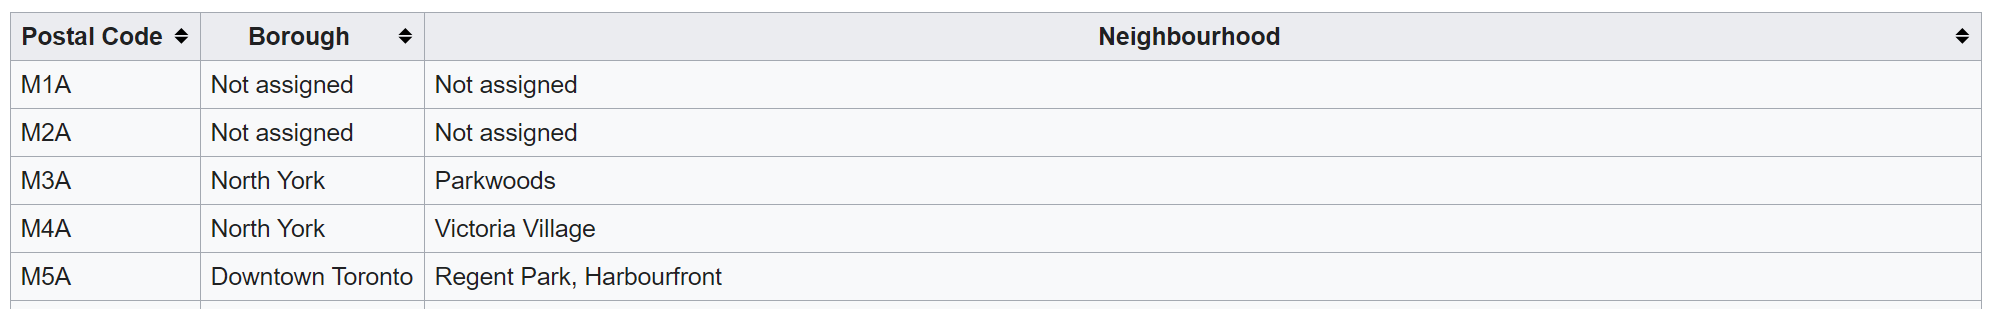
\includegraphics[width=\textwidth]{WikiTable}
         \caption{Wikipedia table view}
         \label{fig: Wiki}
     \end{subfigure}
     \hfill
     \begin{subfigure}[h]{0.45\textwidth}
         \centering
         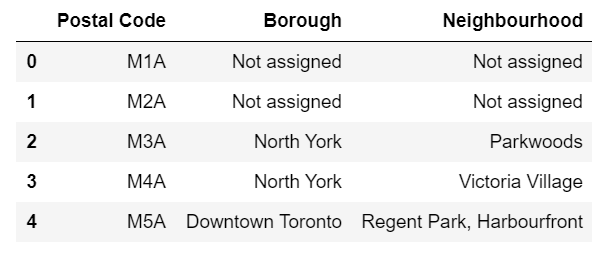
\includegraphics[width=\textwidth]{WikiDf}
         \caption{Extracted dataframe of wikipedia table}
         \label{fig: Wikidf}
     \end{subfigure}
     \caption{Toronto Neighbourhoods Data tables}
\end{figure}

\subsubsection{Preprocessing the Neighbourhoods Data}
With the data having been imported correctly, it now must be preprocessed before any modelling and analysis can be done. The first step is to drop all rows from the table where the boroughs are \textit{Not assigned}. The next step is to assign all \textit{Not assigned} neighbourhoods the value of their respective boroughs. Figure~\ref{fig: Preproc} shows the table after being preprocessed and ready for assigning the respective longitude and latitude values to each location.

\begin{figure}[!h]
\center
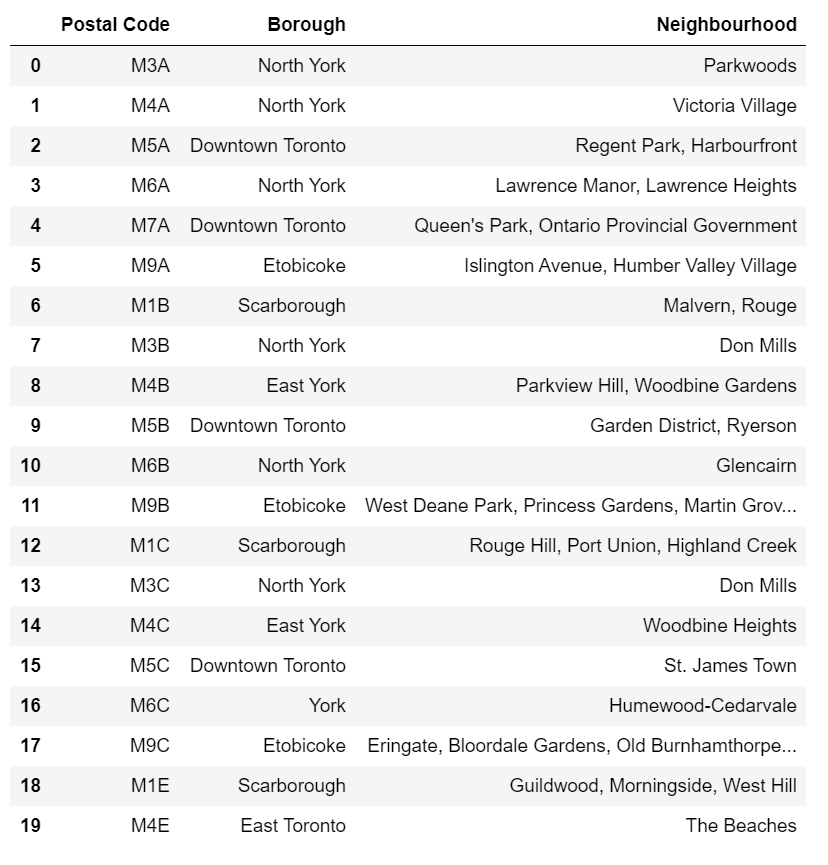
\includegraphics[scale=0.8]{Preproc}
\caption{Neighbourhoods dataframe after being preprocessed}
\label{fig: Preproc}
\end{figure}

\subsubsection{Geospatial Data}
The Geospatial data is the data that will provide the geographical coordinates to the neighbourhoods, specifically the centre point of each neighbourhood. The data is stores in a \textit{csv} file, and is read in as such and converted into a dataframe. Subsequently, this data must be merged with the neighbourhoods dataframe for the data to be modelled and analysed. A left join is done on the neighbourhoods table with the geospatial data table and the resulting dataframe can be seen in Figure~\ref{fig: Finaldf}.

\begin{figure}[!h]
\center
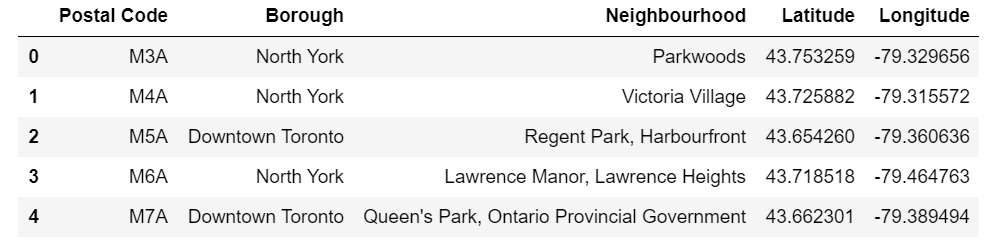
\includegraphics[scale=0.8]{Finaldf}
\caption{Merged dataframe containing Neighbourhoods data}
\label{fig: Finaldf}
\end{figure}

\subsubsection{Demographics data (Used for in-depth analysis)}
The demographics data is a \textit{csv} file that was extracted from the Toronto open Data Catalogue and contained data from a 2016 census. With the amount of information in this file only two rows were extracted, specifically the population of the neighbourhoods and the average income of the neighbourhoods. This data was read in, preprocessed and merged with the Neighbourhoods dataframe. The resulting table can be seen in Figure~\ref{fig: InDepth}.

\begin{figure}[!h]
\center
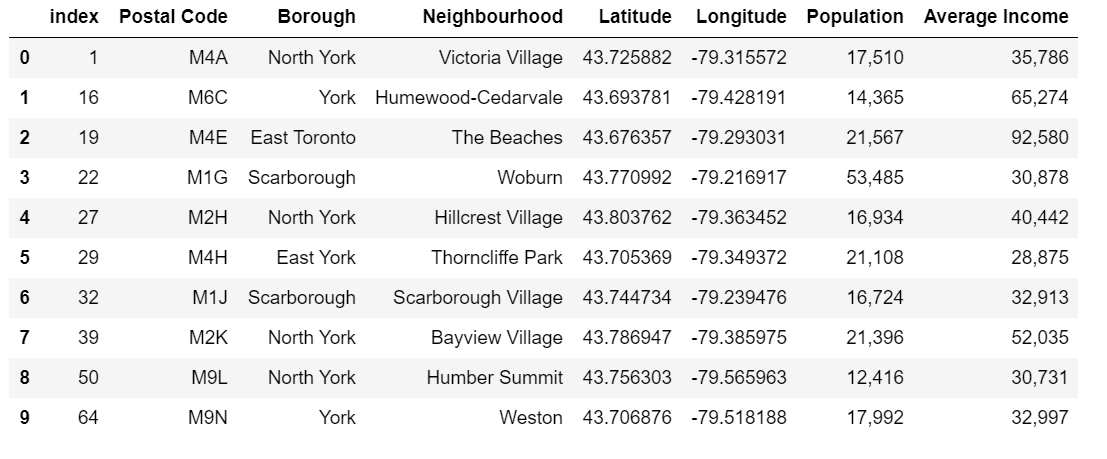
\includegraphics[scale=0.8]{InDepthTable}
\caption{Dataframe used for the in-depth analysis}
\label{fig: InDepth}
\end{figure}

\subsection{Creating the Map}
In order to generate an interactive map with points over each neighbourhood, the \code{folium} and \code{geopy} libraries are used. The \code{geopy} retrieved the centre coordinates of the city of Toronto, and the \code{folium} library is able to take the data from the dataframe as well as the location of Toronto and map it out accordingly as seen in Figure~\ref{fig: Toronto}

\begin{figure}[!h]
\center
\includegraphics[scale=0.35]{TorontoMap}
\caption{Generated map of Toronto and respective neighbourhoods}
\label{fig: Toronto}
\end{figure}

\subsection{Retrieving the venues}
With half of the data ready for modelling and analysis, we can now extract the data required from the Foursquare API. The initial step is to set up your Foursquare credentials in order to retrieve the requested information. Once authenticated, 100 venues within a 500 metre radius of each neighbourhood. This data is requested as a JSON file and once received is converted into a dataframe which can be seen in Figure~\ref{fig: Venues}.

\begin{figure}[!h]
\center
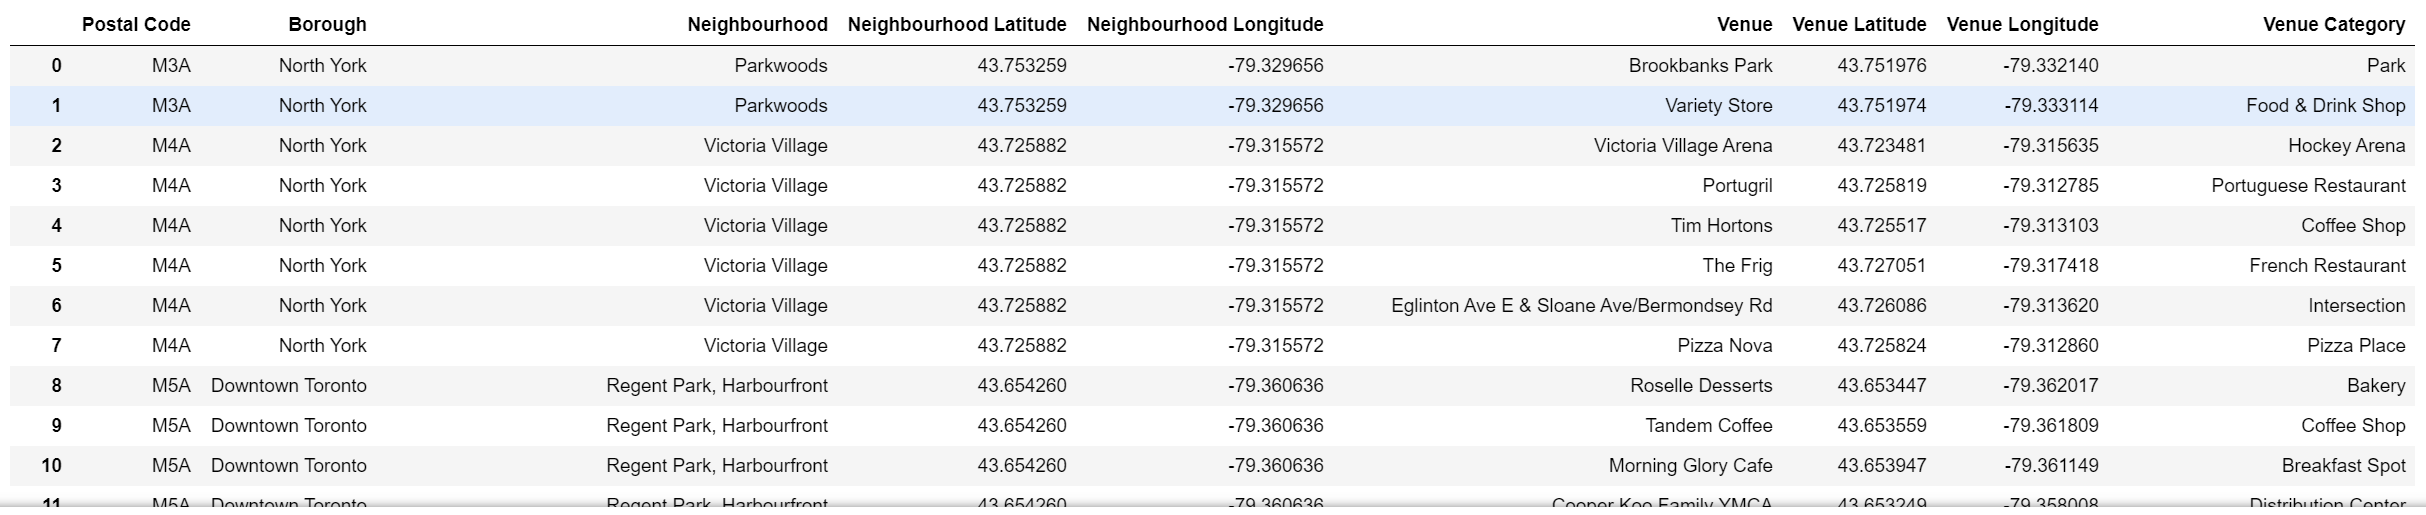
\includegraphics[scale=0.5]{Venuesdf}
\caption{Dataframe of the neighbourhoods and requested venues}
\label{fig: Venues}
\end{figure}

\subsubsection{Grouping the Venues}
All the venues within the requested radius has been presented, however in order to gain a full understanding of the data, the venues are grouped and counted. This is to observe what are some of the popular venues within the city of Toronto. The results can be seen in Figure~\ref{fig: GroupedVenues} which amounts to a total of 273 unique categories of venues. Since no dictionary or classification is done on the venue categories, a café and a coffee shop and a breakfast place are all categorised as unique venues, which for this project was an accepted trade off.

\begin{figure}[!h]
\center
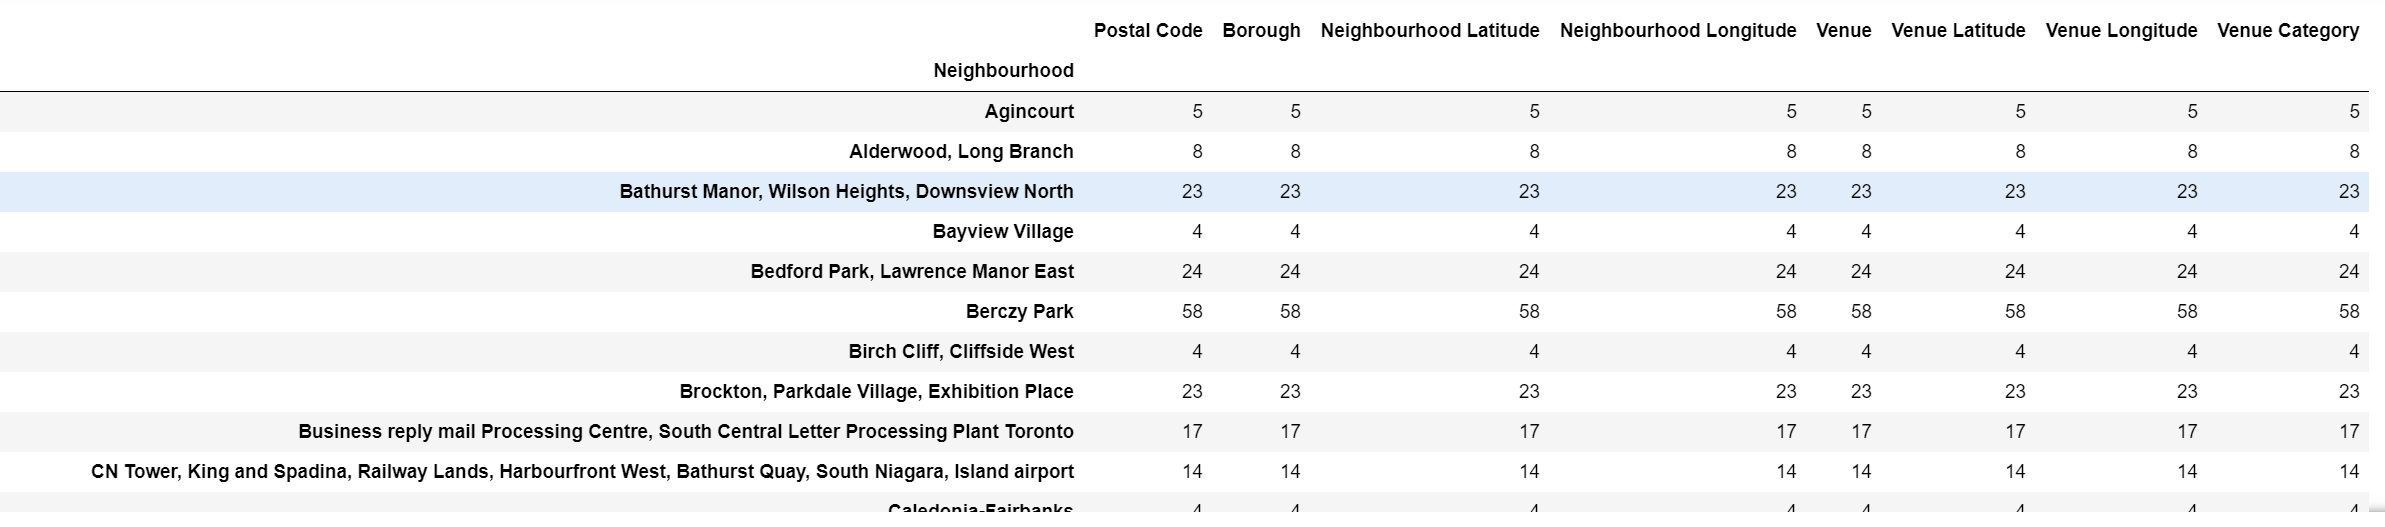
\includegraphics[scale=0.5]{GroupedVenues}
\caption{Dataframe of the venues and the number of times it has appeared in the request}
\label{fig: GroupedVenues}
\end{figure}

\subsection{One Hot Encoding}
One Hot Encoding is a process where categorical variables can be converted in order for a machine learning algorithm to process the data~\cite{OHE}. This converts the variables into a binary format, where a 0 indicates no occurrence and a 1 indicates an occurrence of that respective variable. Figure~\ref{fig: OHE} shows the venues dataframe after being passed through the \code{onehot} function.

\begin{figure}[!h]
\center
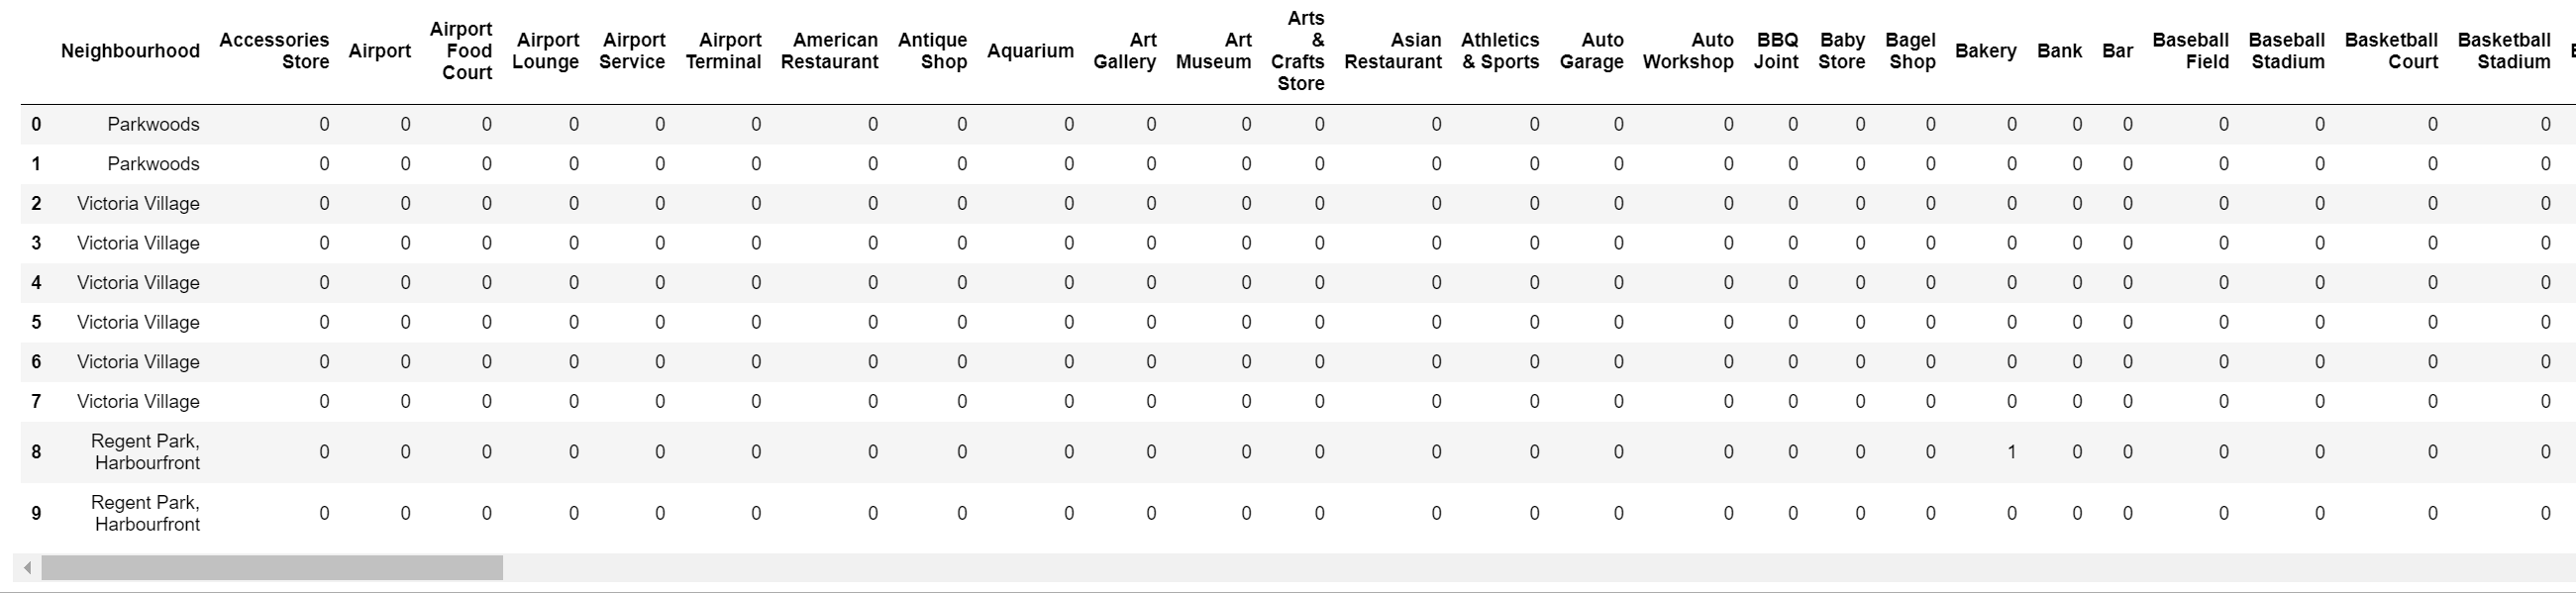
\includegraphics[scale=0.45]{OHE}
\caption{One Hot Encoded dataframe}
\label{fig: OHE}
\end{figure}

\subsubsection{Calculating the average occurrence of each venue}
Once processed and done, One Hot Encoding simply states if that categorical variable, in this case a venue, is present in that neighbourhoods radius. It does not give an indication of how many times that specific venue occurs in the radius. In order to achieve this, the neighbourhoods are grouped and the means of each venue is calculated as seen in Figure~\ref{fig: VenuesMean}.

\begin{figure}[!h]
\center
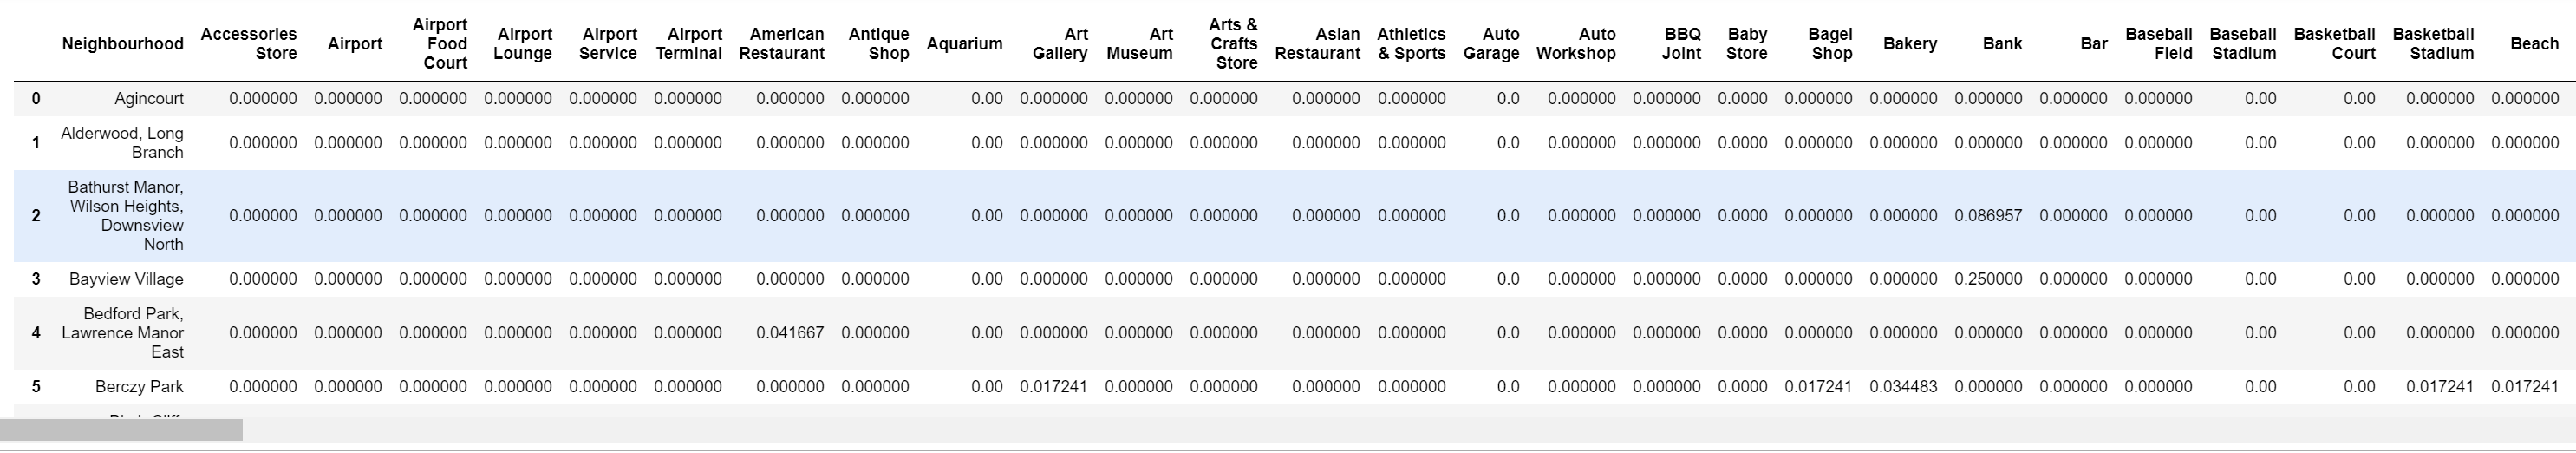
\includegraphics[scale=0.42]{VenuesMean}
\caption{Grouped Neighbourhoods and means of respective venues}
\label{fig: VenuesMean}
\end{figure}

\subsubsection{Presenting the top 10 venues of each neighbourhood}
Now that the means are calculated for each venue for each neighbourhood,the goal is to retrieve the top 10 venues in each neighbourhood to allow investors to see what is the most popular venue categories and what would pose the most competition. Figure~\ref{fig: Top10Ex} displays an example of the top 10 venues of three different neighbourhoods. This raw text data can now be converted into a dataframe for clustering, which can be seen in Figure~\ref{fig: Top10df}.

\begin{figure}[!h]
\center
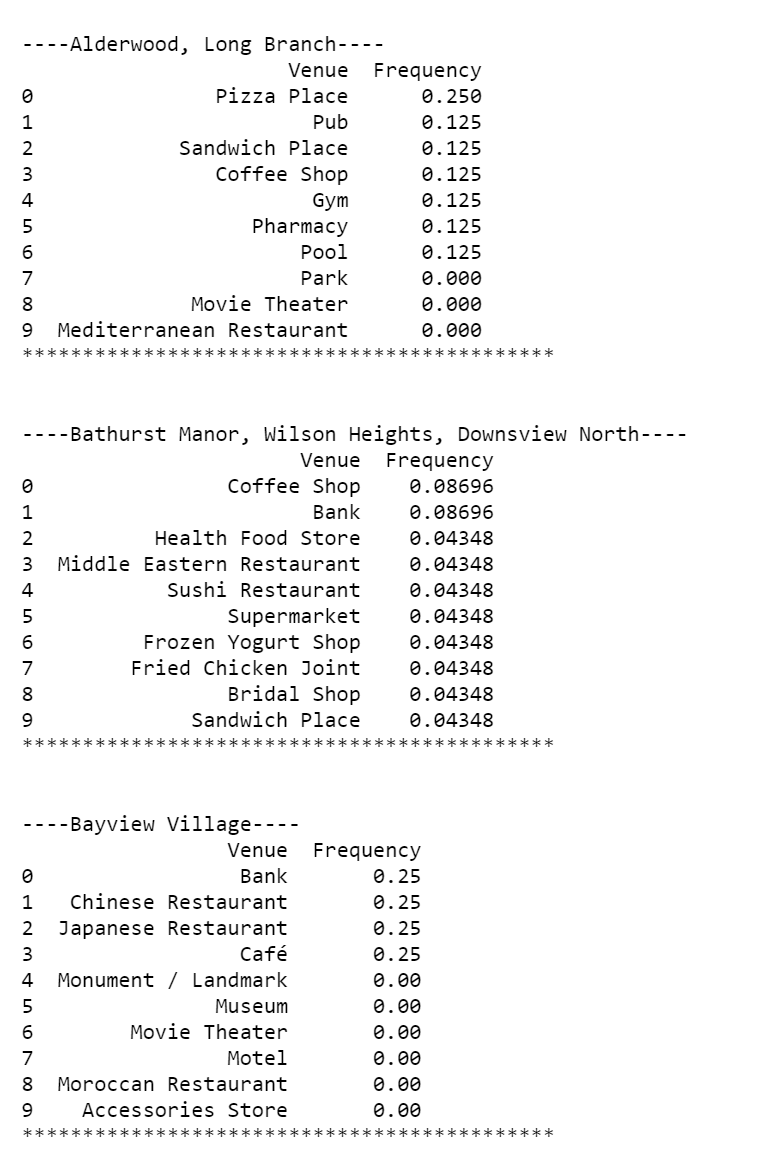
\includegraphics[scale=0.65]{Top10Ex}
\caption{Top 10 venues in various neighbourhoods}
\label{fig: Top10Ex}
\end{figure}

\begin{figure}[!h]
\center
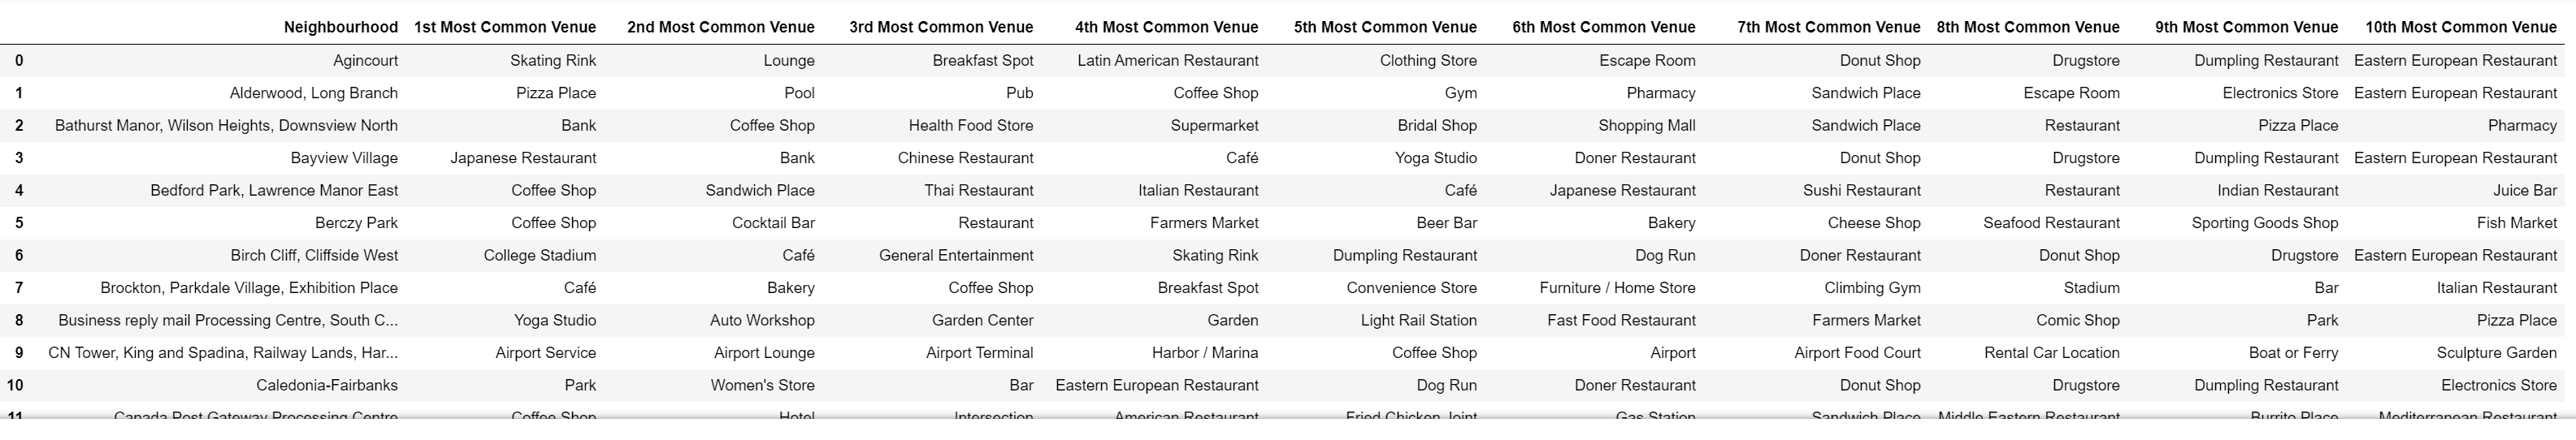
\includegraphics[scale=0.4]{Top10df}
\caption{Dataframe of the top 10 venues in each neighbourhood}
\label{fig: Top10df}
\end{figure}

\subsection{Clustering}
The clustering used in this project is the \textit{k-means} clustering. Five clusters were chosen for the categorisation in order to prevent underfitting and overfitting of the data given the concentration of the various neighbourhoods in the city of Toronto. Figure~\ref{fig: ClusterTable} shows the final processed dataframe after being passed through the machine learning algorithm.

\begin{figure}[!h]
\center
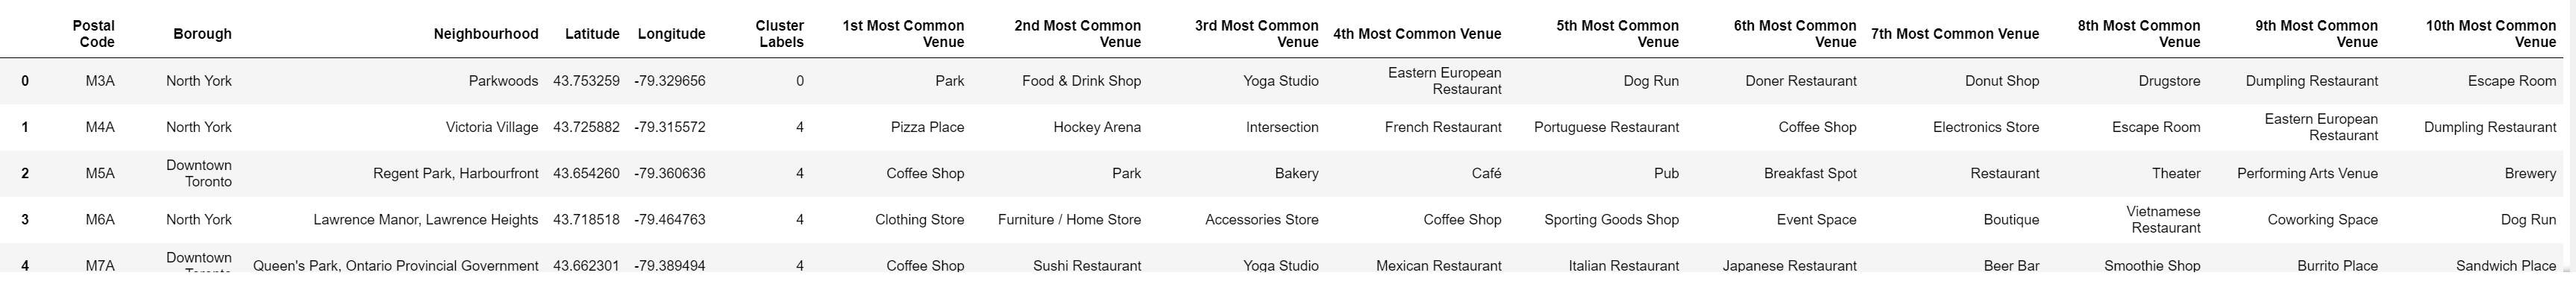
\includegraphics[scale=0.37]{ClusterTable}
\caption{Dataframe of all neighbourhoods, cluster group and top 10 venues}
\label{fig: ClusterTable}
\end{figure}

\section{\textbf{Results}}
\label{sec: Reuslts}

\subsection{Cluster Map}
The neighbourhoods are all clustered, and in order to gain a better understanding on how they were clustered, a map is generated with each cluster being presented in a different colour. Figure~\ref{fig: ClusterMap} displays the map, where the following clusters correspond to the following clusters: gray is cluster 1; black is cluster 2; red is cluster 3; blue is cluster 4; purple is cluster 5.

\begin{figure}[!h]
\center
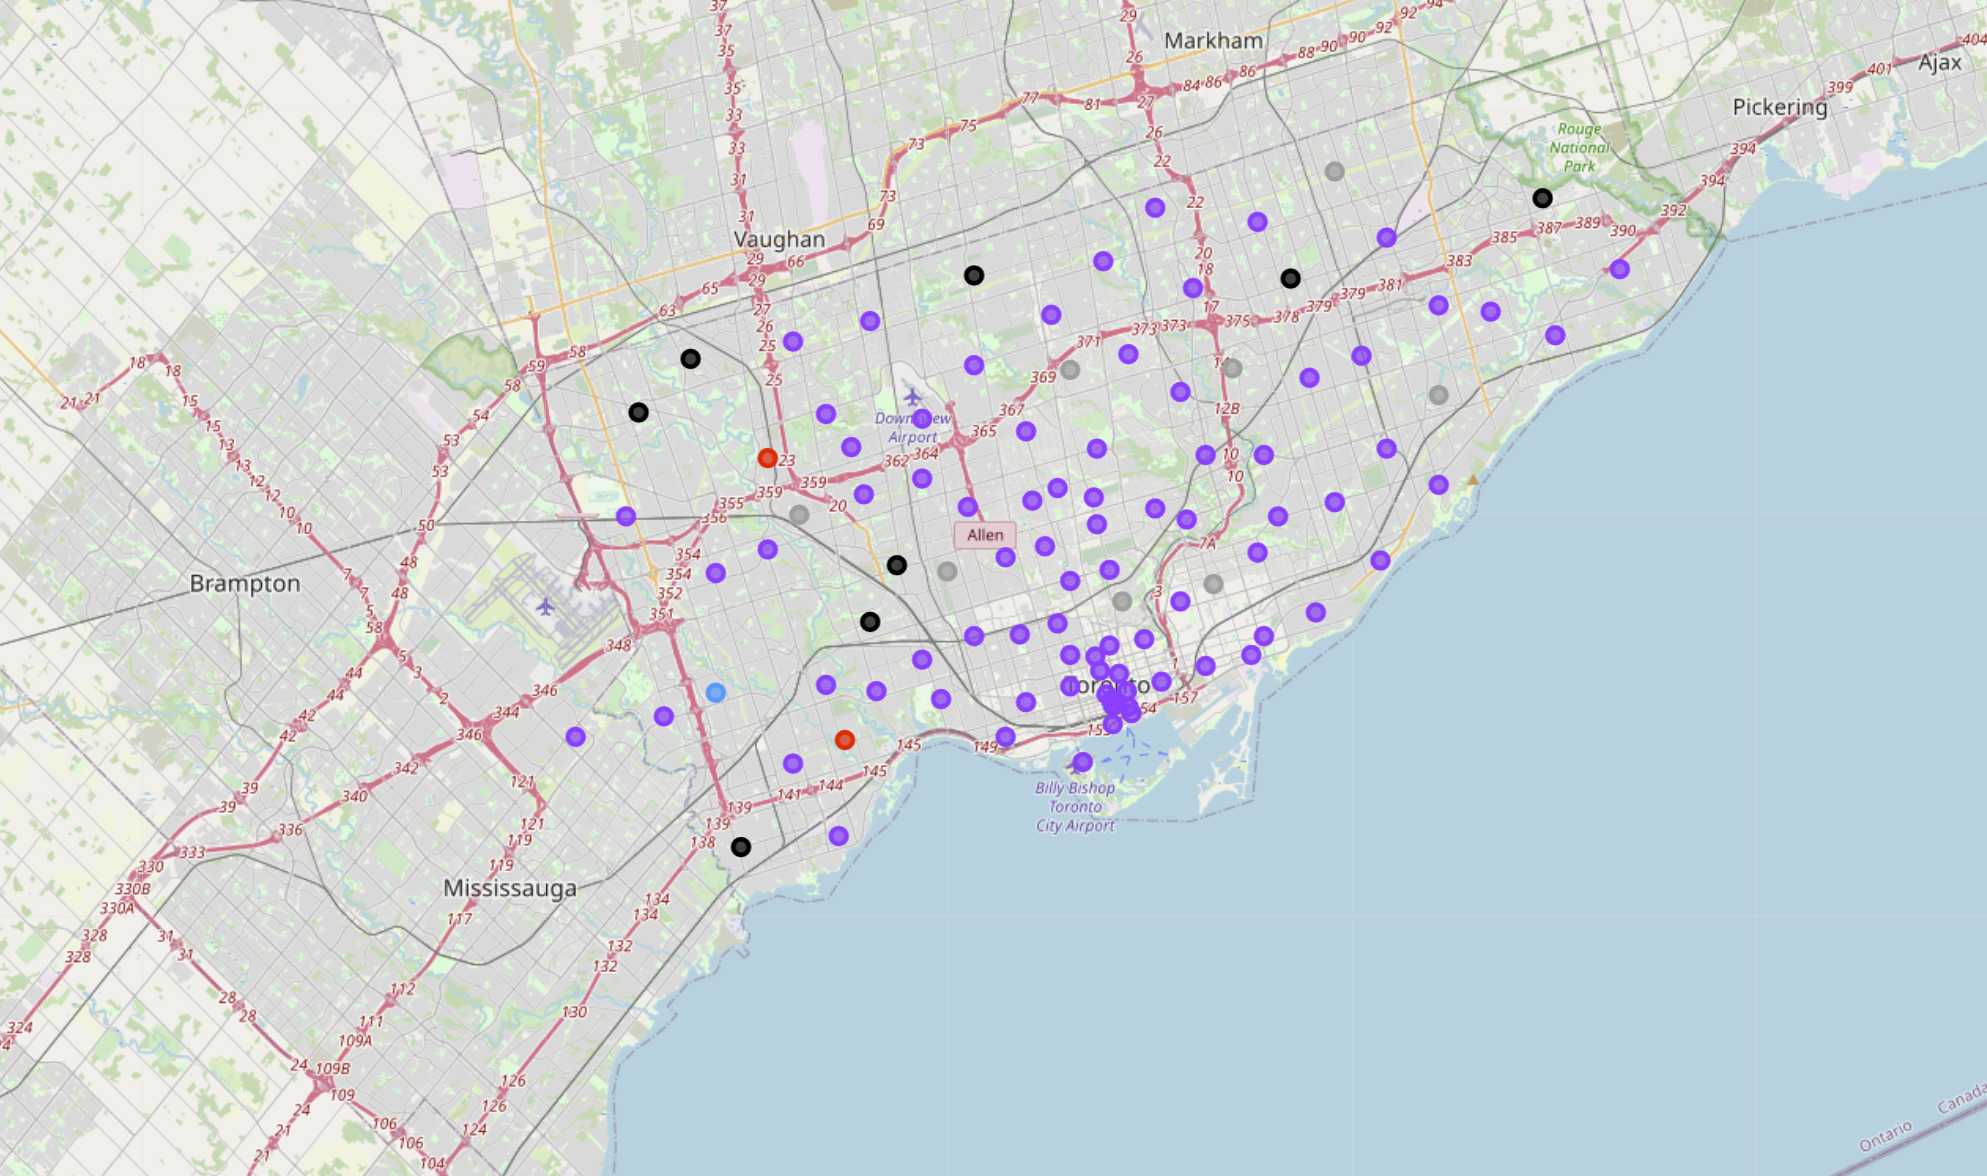
\includegraphics[scale=0.4]{ClusterMap}
\caption{Map showing the clusters}
\label{fig: ClusterMap}
\end{figure}

\subsection{Cluster 1}
If we analyse cluster 1, we can see that based on the most popular venue across all the neighbourhoods are parks and playgrounds. Across the top 10, it seems that all of these neighbourhoods have similarities as the rank of the venues decrease, for example the fifth to the 8th most common venues for the first four neighbourhoods have \textit{Dog run}, \textit{Doner Restaurant}, \textit{Donut shop} and \textit{Drugstore} in the same order.

\begin{figure}[!h]
\center
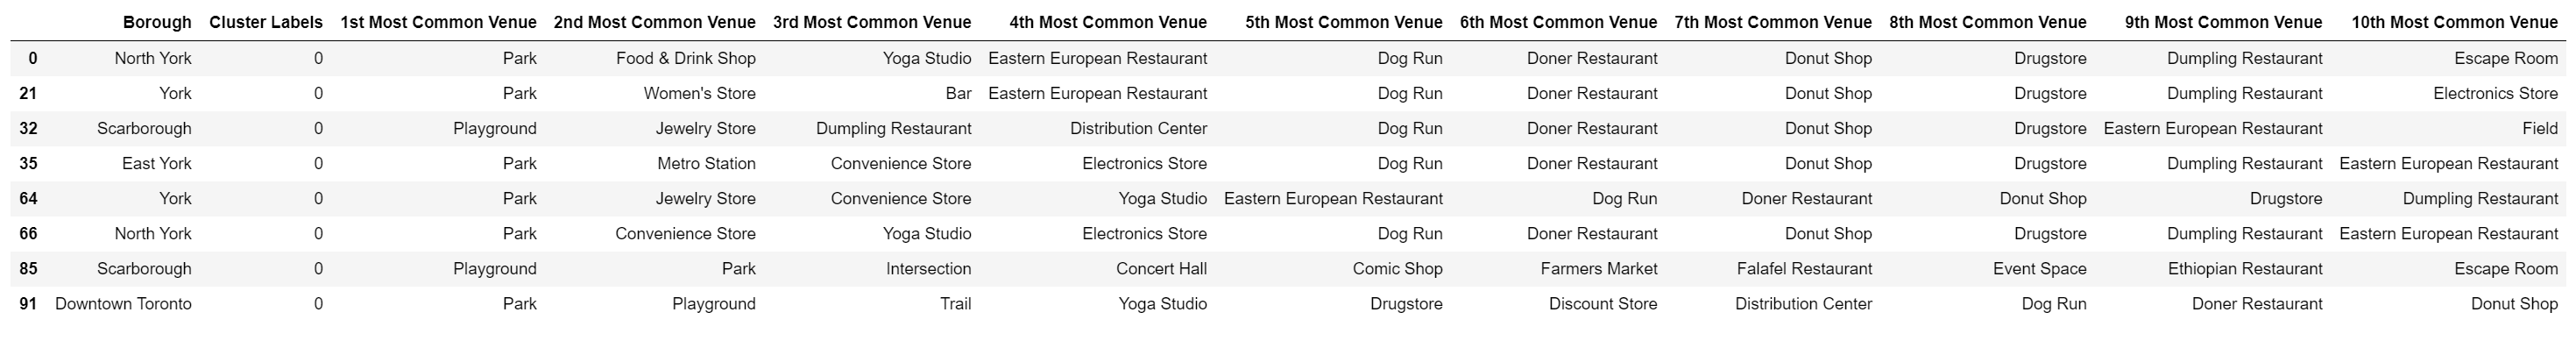
\includegraphics[scale=0.4]{Cluster1}
\caption{Table of cluster 1}
\label{fig: Cluster1}
\end{figure}

\subsection{Cluster 2}
Cluster 2 has a \textit{Pizza place} as it's most common venue in the various neighbourhoods. The various types of restaurants are spread across the rank of each neighbourhood, however almost all exist in each other, albeit at a lower or higher rank. An example of this would be the \textit{Eastern European restaurant} being the third most common venue for the first two neighbourhoods, but the fifth most common venue for the fourth neighbourhood.
\begin{figure}[!h]
\center
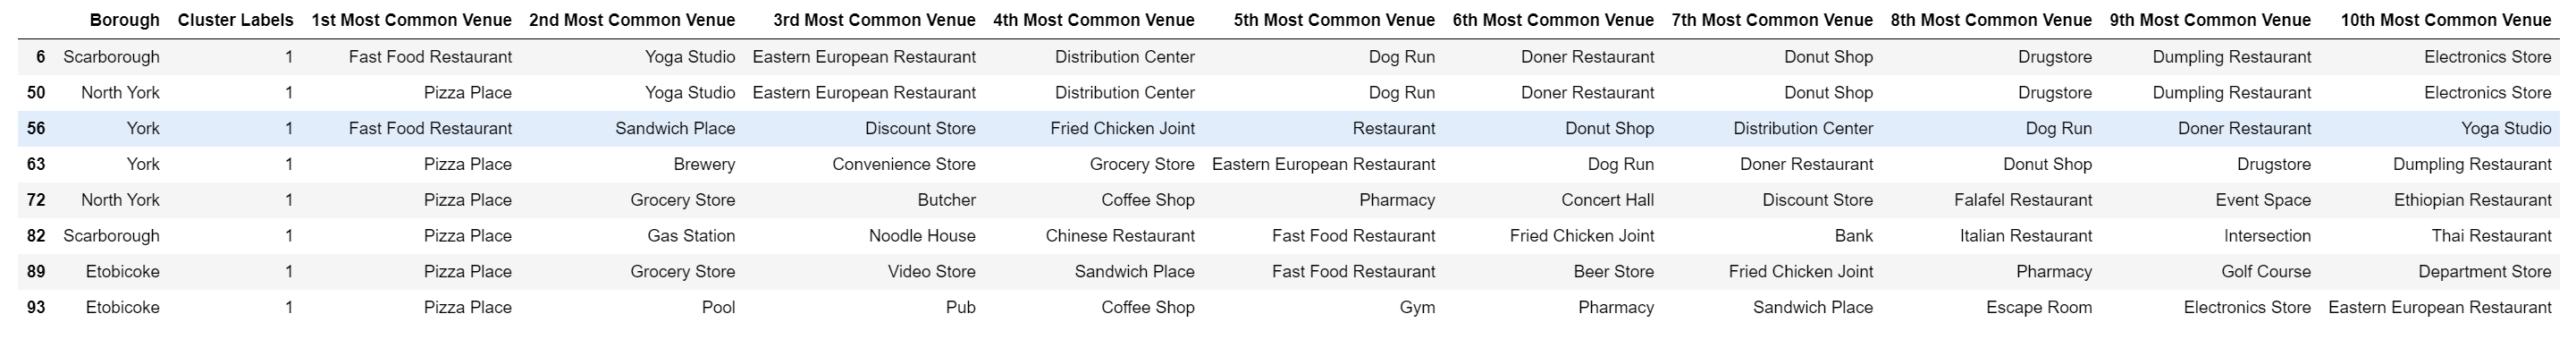
\includegraphics[scale=0.4]{Cluster2}
\caption{Table of cluster 2}
\label{fig: Cluster2}
\end{figure}

\subsection{Cluster 3}
Cluster 3 may not seem to have any similarities with regards to their venues, however these two neighbourhoods are clustered together due to the similarities of their location. Although not regarded as a venue, these two neighbourhoods are situated next to middle schools.
\begin{figure}[!h]
\center
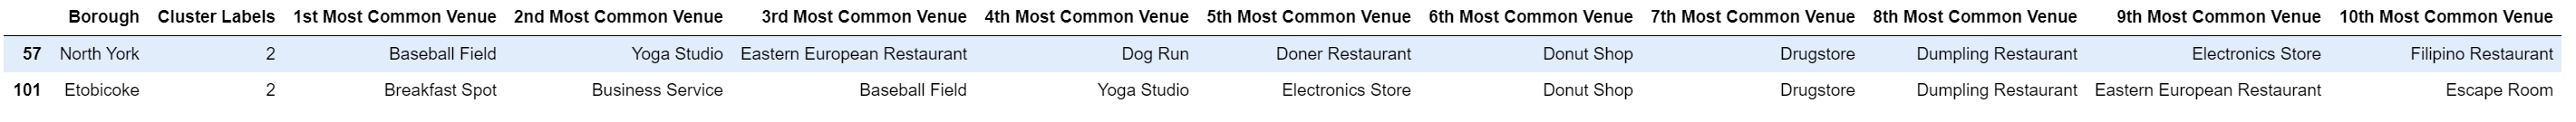
\includegraphics[scale=0.4]{Cluster3}
\caption{Table of cluster 3}
\label{fig: Cluster3}
\end{figure}

\subsection{Cluster 4}
Cluster 4 is somewhat of an outlier as no other neighbourhoods are similar to this, as it's most common venue is a \textit{Filipino restaurant}. As no other cluster has this in common, this neighbourhood is clustered by itself.
\begin{figure}[!h]
\center
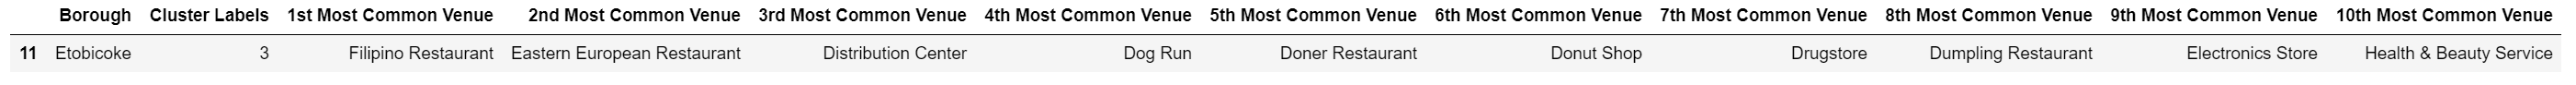
\includegraphics[scale=0.4]{Cluster4}
\caption{Table of cluster 4}
\label{fig: Cluster4}
\end{figure}

\subsection{Cluster 5}
Cluster 5 has the most neighbourhoods in it and shows blatant similarities in the most common venues. These neighbourhoods are clustered together as they are all high-density residential areas.
\begin{figure}[!h]
\center
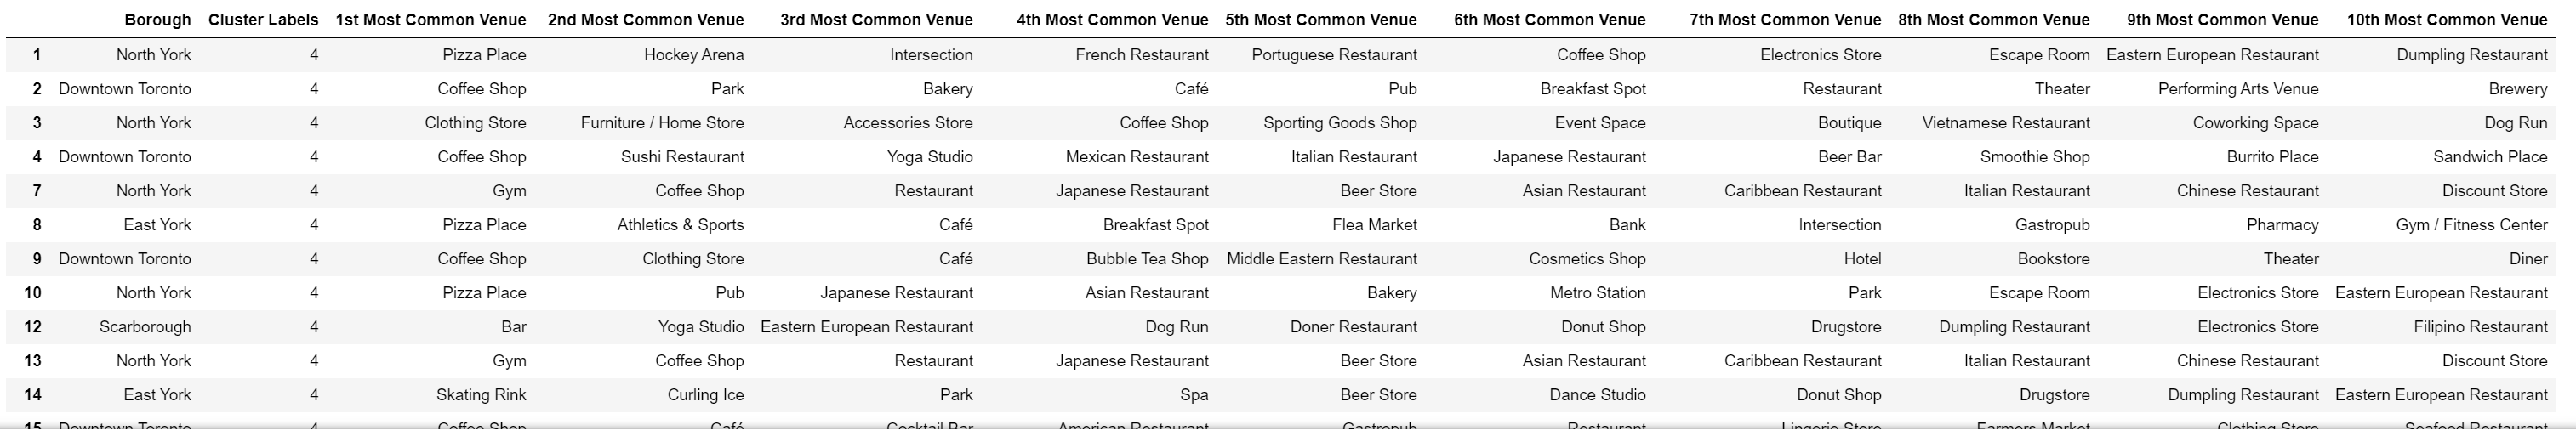
\includegraphics[scale=0.4]{Cluster5}
\caption{Table of cluster 5}
\label{fig: Cluster5}
\end{figure}

\section{\textbf{Discussion \& In-Depth Analysis}}
\label{sec: In-Depth}
For the in-depth analysis, 10 neighbourhoods were chosen and their respective populations and average income was extracted and combined into a single dataframe. These 10 cities will stand as an example to what can be done with this type of clustering and analysis. Figure~\ref{fig: InDepthdf} shows the dataframe of the 10 neighbourhoods while Figure~\ref{fig: InDepthMap} presents the previously clustered neighbourhoods and corresponding clusters.

\begin{figure}[!h]
\center
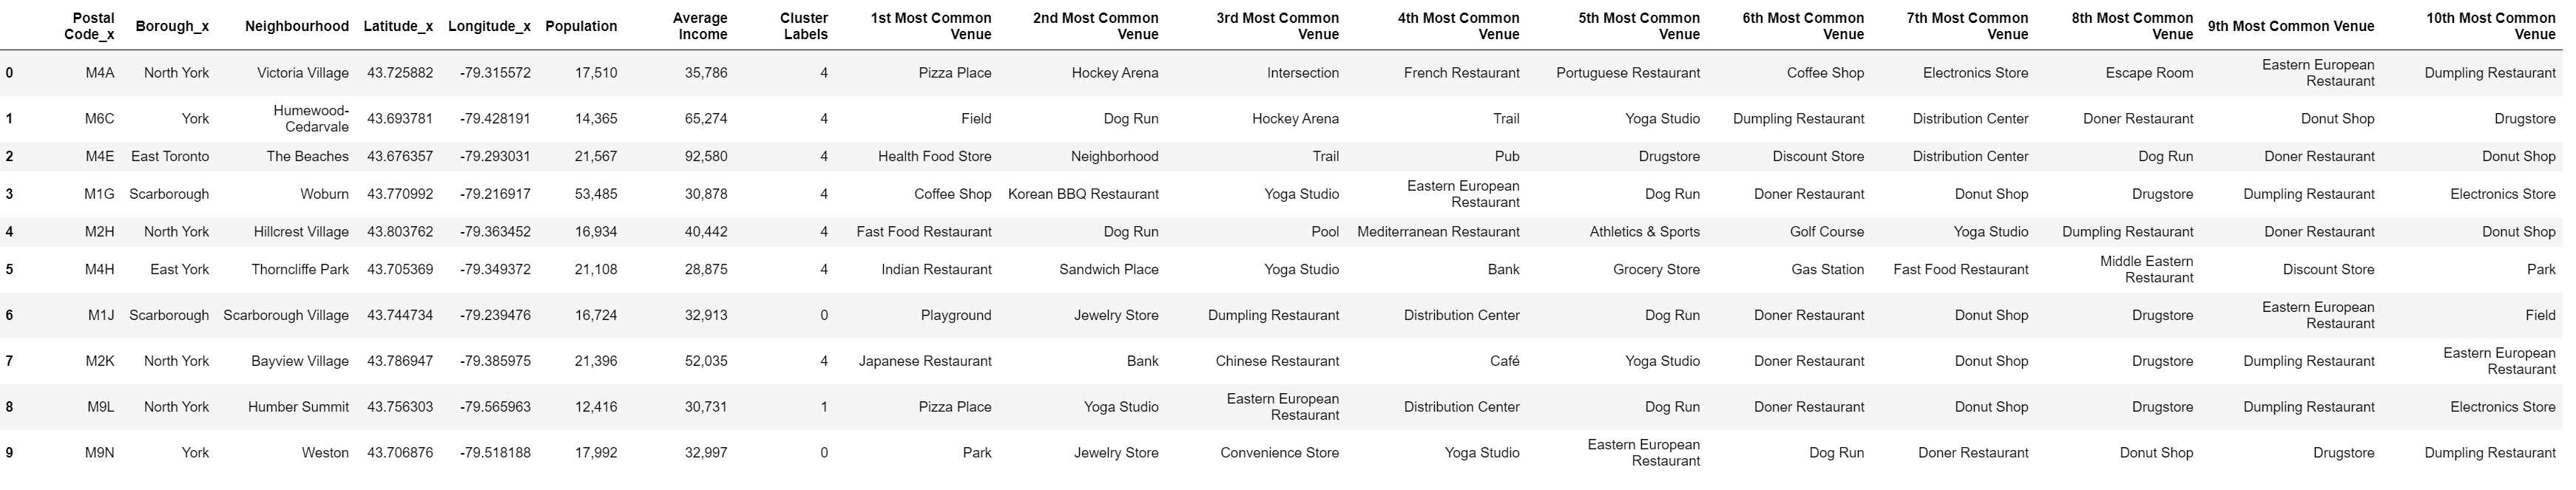
\includegraphics[scale=0.35]{InDepthdf}
\caption{Dataframe of 10 neighbourhoods chosen for in-depth analysis}
\label{fig: InDepthdf}
\end{figure}

The main analysis would rather happen from the dataframe as the pertinent data is presented. If we take the second neighbourhood, \textit{Humewood-Cedervale}, for example we can analyse the following:

\begin{itemize}
\item The neighbourhood is in the fifth cluster, meaning it is in a residential area.
\item The top five most common venues are all healthy or sport related venues.
\item There is no healthy restaurant or healthy food store in the top 10 most common venues.
\item Given the smaller population size, but with the second highest average income in this list, it could stand that a venture capitalist may see an opportunity to invest in a healthy food store that already exists in the area to begin a small franchise.
\item Increasing the number of same-branded healthy food stores can result in more people having access to the stores and make it potentially the sixth most common, if not one of the top five most common venues in the neighbourhood.
\end{itemize}

If we take the \textit{Woburn} neighbourhood, with the largest population size in the list, and one of the lowest average income, we can deduce that this neighbourhood could be a potential location to open a fast food restaurant. However, in the borough of \textit{Scarborough}, the population is potentially ethnically diverse given the various restaurants seen in the top 10 most common venues.

\begin{figure}[!h]
\center
\includegraphics[scale=0.35]{InDepthMap}
\caption{Map of 10 neighbourhoods chosen for in-depth analysis}
\label{fig: InDepthMap}
\end{figure}

This implementation of this project can be drastically improved by utilising more data from the census file such as the ethnicity of people that live in the various neighbourhoods. Furthermore, the overall model can be improved by finding the optimal number of clusters and with increased usage of the Foursquare API, a user can map each neighbourhood's population as a chloropleth, while adding markers to the various venues that are present.

\section{\textbf{Conclusion}}
\label{sec: Conclusion}
A project was implemented on analysing data of the city of Toronto relating to its neighbourhoods. The data was sourced from various locations, preprocessed and presented accordingly. The data was then modelled and clustered using the k-means clustering machine learning algorithm, and an analysis was done on the results. An in-depth analysis was done given more information such as population and average income of the neighbourhood to answer the problem posed in this project. Overall, the project was successful but can stand to be improved with recommendations being given.


\begin{thebibliography}{}

%**************************Section**************************%

\bibitem{VC}
Ganti, A; \textit{Venture Capitalist (VC) Definition}; \url{https://www.investopedia.com/terms/v/venturecapitalist.asp#:~:text=A\%20venture\%20capitalist\%20(VC)\%20is,have\%20access\%20to\%20equities\%20markets}; Last Accessed: 15/01/2021


\bibitem{OHE}
Vasudev, R; \textit{What is One Hot Encoding? Why and When Do You Have to Use it?}; \url{https://hackernoon.com/what-is-one-hot-encoding-why-and-when-do-you-have-to-use-it-e3c6186d008f}; Last Accessed: 15/01/2021

\end{thebibliography}




% that's all folks
\end{document}


